\section{Aufbau}

\begin{figure}
    \centering
    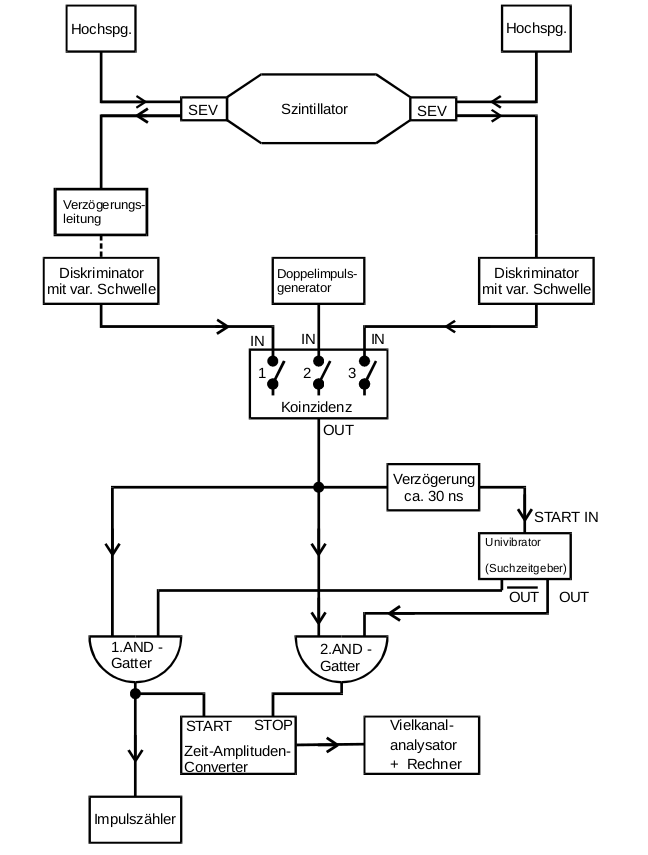
\includegraphics[0.5/\textwidth]{"bilder/aufbau.png"}
    \caption{"Schematischer Aufbau einer Messaperatur um die Drehung durch den Faraday-Effekt zu Messn \cite{skript}."}
    \label{fig:aufbau}
\end{figure}

Der Aufbau beginnt meine einer Halogen-Lampe als Lichtquelle, die also das darauffolgende Element bestrahlt. Das 
emittierte Spektrum einer solchen Lampe befindet sich größtenteils im infraroten Bereich, was den Halbleiter und ihrer 
Resonanzfrequenz gut entgegen kommt. Mit einem Kodensor, also einer Sammellinse, wird das Licht eingefangen und so gebrochen, 
dass das Licht nun parallel zur optischen Achse der Sammellinse weiterläuft. 
Die Lichtquelle wird genau im Brennpunkt des Kondensors platziert, um dessen Funktion zu garantieren.
\\
\newline
In einem darauffolgende \enquote{Lichtzerhacker} wird durch Modulation weitesgehend vermieden, dass weitere leuchtende Quellen im Raum
auf das Empfängersignal einwirken. Die bis hierhin modifizierten Lichstrahlen werden anschließend in einem
\enquote{Glan-Thompson-Prisma} aus Kalkspat gebrochen. \\
Ein solches, doppelbrechendes Prisma ist in der Lage unpolarisiertes Licht zu Polarisieren. Dadurch entsehen 
aus einem Lichtstrahl, zwei weiter mit senkrechtzueinander stehender Polarisatton. Enzig der erzeugte Strahl, 
der parallel zur optischen Achse läuft wird verwendet. Unterstützt wird der Verlauf dieser Achse durch eine metallischen Schiene,
auf der die einzlnen Elemente montiert werden können.
\\
\newline
Ein Konstantstromgerät, mit der Möglichkeit die Polung zu ändern, ist an einem Elektromagneten angeschlossen um ein konstantes (durch Gleichstrom) Magnetfeld
zu erzeugen. Dieses Magnetfeld soll später eine Probe umschließen und möglichst gleichmäßig darum verteilt sein. Damit die Verteilung 
auch bei Eingriffen in den Aufbau möglichst konstant bleibt, bietet es sich an den Magneten mit auf die Schiene zu bauen. Eine Einbuchtung 
darin lässt die einzelnen Proben einführen. Diese sind dort senkrecht zum Lichtstrahl fesgehalten, der wiederum ungehindert zwischen den Hälften des Magneten 
strahlen kann. Die Probe, in der schließlich der Farady-Effekt stattfindet, weist eine relativ hohe Dichte auf, weswegen viel Intensität des Lichtes verloren geht. 
So ist die Wahl vom nötigen Interferenzfilter weitesgehend limitiert auf eine Stelle, nachdem die Strahlen durch die Probe gelangt sind. 
Gewählt wurde im Aufbau eine Platzierung des Filters direkt hinter dem Magneten. Das Licht erfährt ab hier keine weiteren Intensitätsverluste und kann hier problemlos
auf die gewollte Wellenlänge angepasst werden.
\\
\newline
Um das nun linear Polarisierte -und zudem gedrehte Licht auswerten zu können, Bedarf es noch ein weiteres Doppelprisma, welches wieder auf der optischen Achse, also der Schiene,
montiert wird. Hier wird das Licht entsprechend der Ausrichtung der Polarisatton 

